\documentclass[11pt,a4paper]{article}
\usepackage[utf8]{inputenc}
\usepackage[T1]{fontenc}
\usepackage{lmodern}
\usepackage{textcomp}
\usepackage{amsmath,amssymb}
\usepackage{graphicx}
\usepackage{booktabs}
\usepackage{longtable}
\usepackage{array}
\usepackage{listings}
\usepackage{xcolor}
\usepackage[margin=1in]{geometry}
\usepackage{float}
\usepackage[hidelinks,breaklinks]{hyperref}
\usepackage{microtype}
\setlength{\parskip}{4pt}
\lstset{basicstyle=\ttfamily\scriptsize,breaklines=true,breakatwhitespace=false,
  postbreak=\mbox{\textcolor{gray}{$\hookrightarrow$}\space},frame=single,
  framerule=0.3pt,rulecolor=\color{gray!60},columns=fullflexible,keepspaces=true,
  showstringspaces=false,numbers=none,xleftmargin=4pt,xrightmargin=4pt,
  literate={\_}{{\_}}1}
\graphicspath{{figures/}}
\providecommand{\tightlist}{}
\title{Baryonic Suppression of the z=0 Matter Power Spectrum: HACC Emulator Predictions and Literature Assessment}
\author{HEP-Genesis-Agent session record \\ \small Project: ramp-combo-baryonic-pk}
\date{2026-10-17}
\begin{document}
\maketitle
\noindent\textit{\small This document is an AI-generated account of an interactive session with the HEP-Genesis agent. Its text was written by a language model strictly from the session record; figures and numbers come only from tool results obtained during the session. The supplementary material and the transcript, generated alongside, document exactly what ran. Verify independently before use.}
\vspace{1em}

\begin{abstract}
We report a session that combined emulator predictions with a literature survey of baryonic suppression of the matter power spectrum. We used the HACC hydrodynamics emulator to predict the ratio $P_{\rm hydro}(k)/P_{\rm grav}(k)$ at $z=0$ at six points of its seven-parameter design space, with cosmology fixed at $\omega_m=0.14$ and $\sigma_8=0.8$. At $k\simeq1\,h\,{\rm Mpc}^{-1}$ the suppression ranges over the sampled points from an enhancement of $0.2\%$ (weak AGN/kinetic feedback) to $2.92\pm0.15\%$ (lowest wind coupling, $\kappa_w=2$). At $k\simeq3\,h\,{\rm Mpc}^{-1}$ the largest sampled suppression is $10.93\pm0.54\%$. In every run that shows suppression, it is still deepening at $k\simeq3.7\,h\,{\rm Mpc}^{-1}$, the largest wavenumber that could be read from the output. The suppression minimum was therefore not resolved.

All sampled points are consistent with the HSC-XXL gas-fraction constraint of $5\pm4\%$ at $k=1\,h\,{\rm Mpc}^{-1}$. All fall short, by about $3.5\sigma$, of the eROSITA+kSZ preference of $10\pm2\%$ (arXiv:2512.02954). The comparison at $k=3\,h\,{\rm Mpc}^{-1}$ with the cluster-calibrated value of $18.4\%$ (arXiv:2309.02920) shows a factor of about 2 deficit, but this comparison was contested during the session.

From the papers read, AGN-driven gas redistribution in groups and clusters causes the suppression, and lower cluster gas fractions and jet-mode feedback strengthen it. Reconciling KiDS-1000 or DES Y3 shear with Planck through non-linear suppression alone requires suppression stronger, and reaching larger scales, than current simulations produce. FLAMINGO judges it unlikely that baryons drive the $S_8$ tension. No lensing observable was computed.
\end{abstract}

\section{Introduction}

The user asked for four things, in this order:
\begin{enumerate}
\item a survey of recent work on baryonic suppression of the matter power spectrum;
\item emulator predictions of the $z=0$ power-spectrum ratio at a couple of parameter points, using the available hydrodynamics emulator tools;
\item an explanation of the AGN feedback physics responsible for the suppression;
\item an assessment of the impact on weak-lensing cosmology.
\end{enumerate}

The assistant organised the work into seven lines of investigation:
\begin{itemize}
\item emulator predictions at fiducial, strong-AGN and weak-AGN points;
\item a cited synthesis of the feedback physics;
\item robustness and sensitivity checks with the emulator;
\item a cited synthesis of the weak-lensing impact;
\item a reduced, budget-limited parameter-sensitivity study that replaced the full robustness study;
\item closing literature sourcing gaps and cross-checking against published calibrated amplitudes;
\item sourcing the cosmic-shear scale range, the DES Y3 suppression amplitude and a second mitigation method.
\end{itemize}
The last of these ended blocked.

The scope was limited to $z=0$ and to a fixed cosmology. Redshift evolution, cosmology dependence and the emulator's gas-fraction observable were planned but not run. No projected lensing statistic ($C_\ell$ or $\xi_\pm$) was computed.

\section{Methods}

\paragraph{Execution.} All computations ran by local execution. The hydrodynamics server exposed 14 emulated observables, including \texttt{Pk-ratio}, \texttt{fGas}, \texttt{HMF} and \texttt{GSMF}.

\paragraph{Emulator design.} For \texttt{Pk-ratio}, the design space has seven parameters. The parameter-description call returned the following meanings and ranges:
\begin{itemize}
\item $\kappa_w$ (AGN wind coupling / wind efficiency): $[2,4]$;
\item $e_w$ (AGN energy efficiency / wind energy fraction): $[0.2,1]$;
\item $M_{\rm seed}$ (black-hole seed mass in units of $10^6\,M_\odot$): $[0.6,2]$;
\item $v_{\rm kin}$ (kinetic feedback velocity in units of $10^4$ km s$^{-1}$): $[0.1,1.2]$;
\item $\epsilon_{\rm kin}$ (kinetic feedback efficiency in units of 10): $[0.02,1.2]$;
\item $\omega_m=\Omega_m h^2$: $[0.12,0.155]$;
\item $\sigma_8$: $[0.7,0.9]$.
\end{itemize}
The assistant recorded that the design comprises 110 simulations in $400\,h^{-1}$ Mpc boxes.

\paragraph{Emulator output.} Each prediction returned 799 $k$ bins as a CSV file with columns $k$, mean ratio and emulator standard deviation. The ratio is defined relative to the emulator's gravity-only spectrum $P_{\rm grav}$. This is not a separately matched dark-matter-only run.

\paragraph{Runs.} Six predictions were made at $z=0$ with $\omega_m=0.14$ and $\sigma_8=0.8$; their parameter values are listed in Table~\ref{tab:points}. The fiducial point is the centre of the parameter ranges, not a calibrated model. The strong and weak points move $e_w$, $v_{\rm kin}$ and $\epsilon_{\rm kin}$ jointly to their upper or lower bounds. The remaining three runs vary one parameter at a time from the fiducial point.

\begin{table}
\centering
\begin{tabular}{lccccc}
\toprule
Point & $\kappa_w$ & $e_w$ & $M_{\rm seed}$ & $v_{\rm kin}$ & $\epsilon_{\rm kin}$\\
\midrule
Fiducial & 3.0 & 0.6 & 1.3 & 0.65 & 0.61\\
Strong AGN & 3.0 & 1.0 & 1.3 & 1.2 & 1.2\\
Weak AGN & 3.0 & 0.2 & 1.3 & 0.1 & 0.02\\
$\kappa_w=2$ & 2.0 & 0.6 & 1.3 & 0.65 & 0.61\\
$\kappa_w=4$ & 4.0 & 0.6 & 1.3 & 0.65 & 0.61\\
$M_{\rm seed}=2$ & 3.0 & 0.6 & 2.0 & 0.65 & 0.61\\
\bottomrule
\end{tabular}
\caption{HACC emulator parameter points evaluated at $z=0$, with $\omega_m=0.14$ and $\sigma_8=0.8$ for all runs.}
\label{tab:points}
\end{table}

\paragraph{Reading the output.} The table loader rejected the CSV header row with a string-to-float conversion error. The files were therefore read with a plain text reader. This reader has no offset parameter and truncates each 799-bin file near $k\simeq3.7\,h\,{\rm Mpc}^{-1}$, so no values at $k=5$ or $10\,h\,{\rm Mpc}^{-1}$ were obtained. In the tool output reproduced in the record, the displayed portion of each CSV ends near $k\simeq0.42\,h\,{\rm Mpc}^{-1}$. Values quoted below at $k\geq0.5\,h\,{\rm Mpc}^{-1}$ therefore rest on the assistant's extraction as posted to the research board. The draft report itself warned that these values could not be checked against the quoted tool output.

\paragraph{Plots.} Two plots were made with the emulator's plotting tools: a three-curve comparison with the fiducial run as reference, and a single fiducial prediction.

\paragraph{Literature.} The literature work used arXiv abstract search and metadata lookup. Full texts were downloaded and read in chunks for arXiv:2410.17109, 2309.07959, 2206.11794, 2512.02954, 2309.02920, 2305.09827 and 2410.12500. Verbatim supporting quotes were stored in a bibliography file for 2309.07959, 2206.11794, 2512.02954, 2410.17109 and 2309.02920. arXiv:2305.09827 and 2410.12500 were read but never entered in that file.

\paragraph{Review.} A critic reviewed the plan, each wave of work and the draft report. Its verdicts were "revise" (plan), "continue" (two waves, contesting several findings) and "revise" (report). The supplement holds the full tool-call log.

\section{Results}

\subsection{Literature survey}

The initial search returned material spanning three groups of work:
\begin{itemize}
\item \textbf{Simulation-based studies:} the OWLS study of galaxy-formation effects on the power spectrum (arXiv:1104.1174); a library of 92 simulation power spectra (arXiv:1906.00968); FLAMINGO baryon-response and $S_8$ papers (arXiv:2410.17109, arXiv:2309.07959); TNG halo-mass decompositions (arXiv:2511.10634, arXiv:2309.06479).
\item \textbf{Observationally calibrated approaches:} cluster-based baryon-correction modelling (arXiv:2309.02920); the joint X-ray, kSZ and galaxy-galaxy-lensing analysis of arXiv:2512.02954; DES Y3 small-scale shear constraints with a baryonic correction model (arXiv:2206.08591).
\item \textbf{Weak-lensing tension and mitigation:} the "non-linear solution" papers (arXiv:2206.11794, arXiv:2305.09827); a halo-profile parametrisation (arXiv:1810.08629); an analytic redshift-independent formulation (arXiv:2504.15633); a theoretical-error-covariance mitigation (arXiv:2410.12500).
\end{itemize}

The assistant's first survey message contains two problems. First, it stated incorrectly that no emulator tool was available; the HACC emulator was in fact used in the next stage. Second, it quoted a characteristic suppression minimum of roughly 10--30\% at $k\sim5$--$20\,h\,{\rm Mpc}^{-1}$ with a high-$k$ upturn. The assistant itself flagged this as general knowledge that was not sourced from the papers read, and it is not treated as a finding here.

\subsection{HACC emulator predictions at $z=0$}

Table~\ref{tab:three} lists the ratio for the fiducial, strong and weak points.

\begin{table}
\centering
\begin{tabular}{lccc}
\toprule
$k$ [$h\,{\rm Mpc}^{-1}$] & Fiducial & Strong AGN & Weak AGN\\
\midrule
0.101 & 0.99968 & 0.99962 & 1.00009\\
0.510 & 0.99197 & 0.99062 & 1.00096\\
0.997 & $0.97832\pm0.00096$ & $0.97506\pm0.00175$ & $1.0023\pm0.0025$\\
2.00 & $0.95104\pm0.00229$ & $0.94463\pm0.00405$ & 1.0089\\
3.01 & $0.91968\pm0.00346$ & $0.91207\pm0.00596$ & 1.0074\\
3.71 & 0.8979 & 0.8904 & $1.0012\pm0.0105$\\
\bottomrule
\end{tabular}
\caption{HACC $P_{\rm hydro}/P_{\rm grav}$ at $z=0$, with emulator $1\sigma$ where it was extracted.}
\label{tab:three}
\end{table}

At $k\simeq1\,h\,{\rm Mpc}^{-1}$ the suppression $1-P_{\rm hydro}/P_{\rm grav}$ is $2.2\%$ (fiducial), $2.5\%$ (strong) and $-0.2\%$ (weak). The negative value means the weak point is enhanced.

The fiducial and strong curves remain monotonically deepening at $k=3.71\,h\,{\rm Mpc}^{-1}$. Their minimum lies at higher $k$ and was not measured.

The weak-feedback point shows no suppression anywhere in the readable range. Its ratio peaks at about $1.0097\pm0.0072$ near $k\simeq2.4\,h\,{\rm Mpc}^{-1}$. The session produced no sourced physical explanation for this enhancement.

Moving $e_w$, $v_{\rm kin}$ and $\epsilon_{\rm kin}$ jointly to their upper bounds changes the $k=1$ suppression by only about $0.3$ percentage points. This shift is comparable to two to three times the emulator $1\sigma$ there, which is $0.1$--$0.25\%$. The weak-to-fiducial difference of $2.4$ percentage points is well resolved.

Figure~\ref{fig:8} overlays the three $z=0$ ratio curves, with the fiducial run as reference. It shows the main physical result of this subsection. Increasing the AGN energy and kinetic parameters deepens the small-scale deficit only marginally relative to the fiducial run. Lowering them removes the deficit entirely and gives a slight excess at $k\sim$ few $h\,{\rm Mpc}^{-1}$.


\begin{figure}[H]
\centering
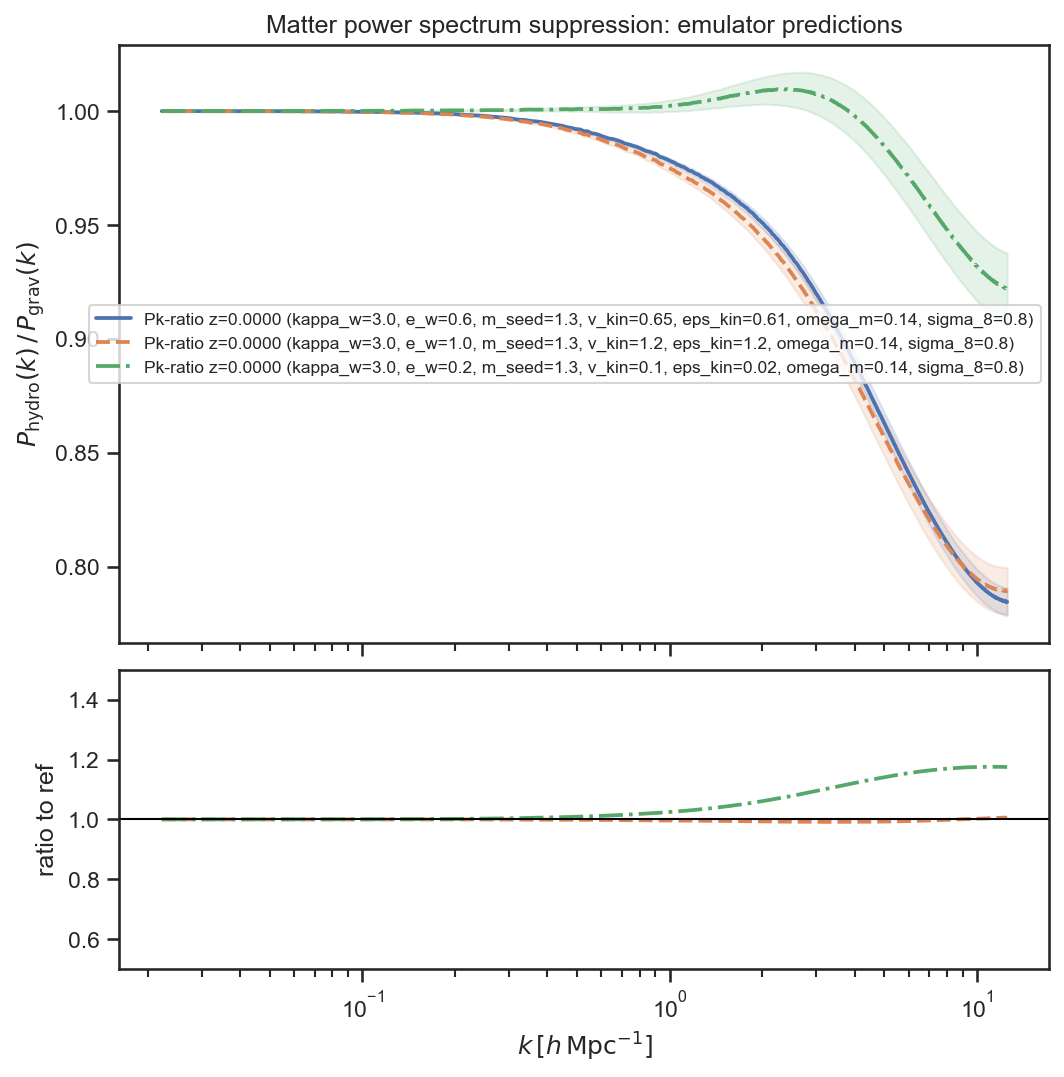
\includegraphics[width=0.85\textwidth,height=0.6\textheight,keepaspectratio]{fig-8.png}
\caption{Pk-ratio\_comparison.png Produced in this session by \texttt{plot\_observable\_comparison} on \textit{serve-hydro.sh}.}
\label{fig:8}
\end{figure}



Figure~\ref{fig:9} shows the fiducial prediction on its own. Within the readable range, the departure from unity is at the $10^{-4}$ level at $k\simeq0.1\,h\,{\rm Mpc}^{-1}$ and grows to about $10\%$ near $k\simeq3.7\,h\,{\rm Mpc}^{-1}$.


\begin{figure}[H]
\centering
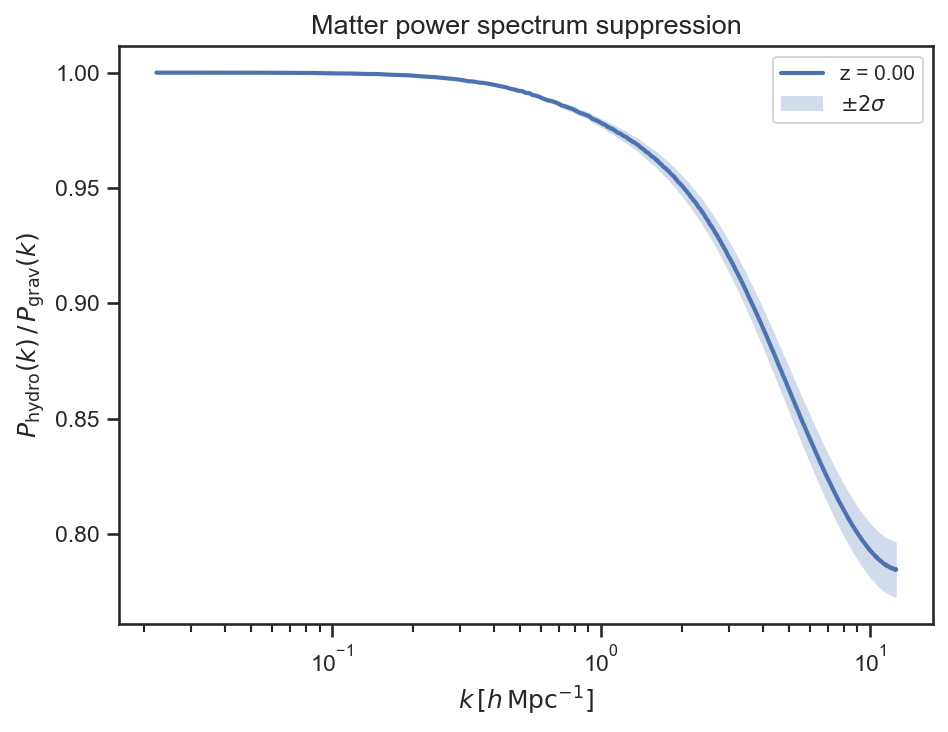
\includegraphics[width=0.85\textwidth,height=0.6\textheight,keepaspectratio]{fig-9.png}
\caption{Pk-ratio\_z0.0000\_prediction.png Produced in this session by \texttt{plot\_prediction} on \textit{serve-hydro.sh}.}
\label{fig:9}
\end{figure}



An initial claim held that the full AGN/kinetic design range spans only about $-0.2\%$ to $+2.5\%$ at $k=1$. The critic contested it, and the $\kappa_w=2$ run later contradicted it. It was replaced by a statement restricted to the sampled points, given in the comparison subsection below.

\subsection{One-at-a-time parameter sensitivity}

Table~\ref{tab:sens} gives the suppression for the $\kappa_w$ and $M_{\rm seed}$ variations, with all other parameters fixed at the fiducial point.

\begin{table}
\centering
\begin{tabular}{lccc}
\toprule
Run & $k=0.997$ & $k=3.007$ & $k=3.714$ [$h\,{\rm Mpc}^{-1}$]\\
\midrule
Fiducial & 2.17\% (0.10\%) & 8.03\% (0.35\%) & 10.2\%\\
$\kappa_w=2$ & 2.92\% (0.15\%) & 10.93\% (0.54\%) & 13.66\% (0.64\%)\\
$\kappa_w=4$ & 1.31\% (0.13\%) & 4.95\% (0.46\%) & 6.60\% (0.54\%)\\
$M_{\rm seed}=2.0$ & 2.42\% (0.14\%) & 9.03\% (0.49\%) & 11.40\% (0.57\%)\\
\bottomrule
\end{tabular}
\caption{Suppression $1-P_{\rm hydro}/P_{\rm grav}$ at $z=0$, with emulator $1\sigma$ in parentheses.}
\label{tab:sens}
\end{table}

Lower wind coupling $\kappa_w$ strengthens the suppression, and a larger seed mass strengthens it mildly. The ranking of shifts from the fiducial point is as follows.
\begin{itemize}
\item At $k=1$: the joint lowering of $(e_w, v_{\rm kin}, \epsilon_{\rm kin})$ gives the largest shift ($-2.4$ percentage points). The full $\kappa_w$ range comes next (1.6 percentage-point spread). The joint raising follows ($+0.33$), and $M_{\rm seed}$ from 1.3 to 2.0 is smallest ($+0.25$).
\item At $k=3$: the ordering is joint lowering (about $-8.8$ percentage points), then $\kappa_w$ (5.98 percentage-point spread), then $M_{\rm seed}$ ($+1.0$), then joint raising ($+0.76$).
\end{itemize}
Every shift at $k=3$ exceeds the emulator $1\sigma$ of $0.35$--$0.54\%$. At $k=1$ the $M_{\rm seed}$ and joint-raising shifts are only about $2\sigma$.

Two limitations apply. First, $e_w$, $v_{\rm kin}$ and $\epsilon_{\rm kin}$ were only moved together, so their individual sensitivities are unknown. Second, $\omega_m$ and $\sigma_8$ were never varied, so the cosmology dependence of HACC was not checked. No comparison plot was made for these three runs, and values at $k\leq0.5\,h\,{\rm Mpc}^{-1}$ were not recorded for them.

\subsection{AGN feedback physics, from the literature read}

The mechanism, as stated in the texts read, is redistribution of gas relative to the dark matter by energy injected by AGN. This suppresses non-linear power by tens of percent relative to dark-matter-only runs (arXiv:2512.02954). Below about 10 Mpc AGN push baryons outward, while on smaller scales star formation concentrates baryons in halo centres (arXiv:2309.02920).

FLAMINGO (arXiv:2410.17109) reports several dependencies of the response:
\begin{itemize}
\item \textbf{Strengthening factors:} lower gas fractions in groups and clusters, collimated jets in place of thermally driven winds, and lower stellar masses at fixed gas fraction.
\item \textbf{Redshift evolution:} the response strengthens and extends to larger scales as redshift falls. In the fiducial model the minimum of $P/P_{\rm DMO}$ moves from $k=6\,h\,{\rm Mpc}^{-1}$ at $z=2$ to $k=10\,h\,{\rm Mpc}^{-1}$ at $z=0$. The departure from unity begins at $k\sim1\,h\,{\rm Mpc}^{-1}$ at $z=2$ and at $k\sim0.1\,h\,{\rm Mpc}^{-1}$ at $z=0$.
\item \textbf{Gas-fraction variants:} for thermal-AGN variants spanning $f_{\rm gas}$ from $-10\sigma$ to $+4\sigma$, the $z=0$ minimum stays at $k=8$--$10\,h\,{\rm Mpc}^{-1}$. The $f_{\rm gas}$ parameter mainly changes the normalisation, and the response saturates below $f_{\rm gas}-8\sigma$, which is an emulator extrapolation.
\item \textbf{Jet model:} it is stronger at negative $f_{\rm gas}$ but has a similar $k$-range and minimum position.
\item \textbf{Cosmology dependence:} about $1\%$ for $k<10\,h\,{\rm Mpc}^{-1}$.
\item \textbf{Emulator accuracy:} better than $1\%$ up to $k=10\,h\,{\rm Mpc}^{-1}$ and $z=3$.
\end{itemize}
The FLAMINGO text gives no number for the depth of the $z=0$ minimum, which appears only graphically in its figures.

This literature synthesis, as first posted, was contested by the critic. The corrected and quoted elements above are those subsequently sourced. One item from the survey text was not separately sourced with quotes: the identification of $10^{13}$--$10^{14}\,M_\odot$ groups and clusters as the dominant halo mass range, with references to arXiv:2309.06479 and arXiv:2511.10634. It should be read as the assistant's statement.

\subsection{Comparison with observationally calibrated amplitudes}

This comparison is a range-of-model check, not a calibration. Cosmology and halo-mass weighting differ between the analyses, and HACC parameters do not map onto FLAMINGO $f_{\rm gas}$ or jet variants. The benchmarks are as follows.
\begin{itemize}
\item arXiv:2512.02954, for haloes with $13<\log_{10}M_{500}<14$ at $0<z<1$: joint eROSITA+kSZ gives $10\pm2\%$ at $k=1\,h\,{\rm Mpc}^{-1}$, and HSC-XXL gas fractions give $5\pm4\%$. Only the strong-feedback BAHAMAS 8.0 and FLAMINGO $f_{\rm gas}-8\sigma$ runs agree with eROSITA+kSZ. The simulations differ from one another by more than $10\%$ at $k=1$.
\item Grandis et al. (arXiv:2309.02920), fiducial baryon-correction model: $0.042^{+0.012}_{-0.014}$ at $k=1$ and $0.184^{+0.026}_{-0.031}$ at $k=3\,h\,{\rm Mpc}^{-1}$. Their alternative model gives $0.049^{+0.016}_{-0.012}$ and $0.179^{+0.018}_{-0.020}$. At $97.5\%$ credibility they find an impact below $1\%$ for $k<0.37\,h\,{\rm Mpc}^{-1}$.
\end{itemize}

At $k=1$ the six sampled HACC points span $-0.2\%$ to $2.9\%$, and none reaches $5\%$. The most suppressed point, $\kappa_w=2$ at $2.92\pm0.15\%$, compares as follows:
\begin{itemize}
\item about $0.5\sigma$ from HSC-XXL;
\item about $3.5\sigma$ short of eROSITA+kSZ, using the observational error only (the strong point is short by about $3.7\sigma$);
\item the fiducial and strong points lie about $1.2$--$1.4\sigma$ below the $4.2\%$ of arXiv:2309.02920.
\end{itemize}

At $k=3$ the fiducial and strong points give $8.0\%$ and $8.8\%$. These are a factor of about $2.1$--$2.3$ below the $18.4\%$ of arXiv:2309.02920, or about $3.1$--$3.4\sigma$ against its lower error bar. The largest sampled value, $10.9\pm0.5\%$ at $\kappa_w=2$, is still about $2.4\sigma$ low. The critic contested this $k=3$ comparison, and the gap was left unexplained.

\subsection{Impact on weak-lensing cosmology}

\paragraph{KiDS-1000.} Amon \& Efstathiou (arXiv:2206.11794) consider KiDS-1000 shear, with $S_8=0.759^{+0.024}_{-0.021}$. They show it can be reconciled with Planck $\Lambda$CDM if non-linear power is suppressed with $A_{\rm mod}\approx0.69$ and the suppression extends to $k\sim0.2\,h\,{\rm Mpc}^{-1}$. That range lies outside the BAHAMAS range. A first board posting described this as the only route; a later correction recorded it as sufficient rather than unique.

\paragraph{DES Y3.} Preston, Amon \& Efstathiou (arXiv:2305.09827) use $P_m=P_L+A_{\rm mod}(P_{\rm NL}-P_L)$. They find that DES Y3 requires suppression "not as strong as inferred using KiDS data" but "still more extreme than predictions from recent numerical simulations". They also note that non-standard dark matter is an alternative interpretation. The numerical DES Y3 $A_{\rm mod}$ lies in body text that was not read and remains unsourced.

\paragraph{FLAMINGO.} FLAMINGO (arXiv:2309.07959) finds across its feedback variants that baryonic effects are not large enough to remove the tension. It states that "it is unlikely that baryon physics is driving this modification".

\paragraph{Mitigation by gas calibration.} Siegel et al. (arXiv:2512.02954) analyse an LSST Y1-like mock. Ignoring baryons biases $S_8$ significantly; the shift is shown only graphically. An uninformed baryonification model removes the bias but roughly halves the precision. A kSZ+eROSITA-calibrated prior recovers about half the lost precision.

\paragraph{Mitigation by theoretical-error covariance.} A second method, Maraio, Hall \& Taylor (arXiv:2410.12500), replaces binary $\ell$ scale cuts with a theoretical-error covariance in $P(k)$. For a Euclid-like survey with $\ell_{\rm max}=5000$, the abstract reports that this reduces the bias in $\Omega_m$ and $S_8$ to acceptable levels with a modest increase in variance. This finding rests only on the abstract and was contested by the critic. The only shear scale range sourced in the session is that baryon-sensitive shear extends to $\ell\sim5000$; no $\theta$ range was sourced.

\paragraph{HACC against the required suppression.} An approximate comparison set the HACC suppression against the suppression these analyses require. HACC gives about $0.03$--$0.04\%$ at $k=0.1$, $0.8$--$0.9\%$ at $k=0.5$ and at most $2.5$--$2.9\%$ at $k=1\,h\,{\rm Mpc}^{-1}$. The $A_{\rm mod}$-type suppression reaching $k\sim0.2\,h\,{\rm Mpc}^{-1}$ is far larger. This comparison was also contested, and it involves no projected lensing statistic.

\section{Discussion}

The HACC emulator yields a modest $z=0$ suppression over its sampled design points, at most about $3\%$ at $k=1\,h\,{\rm Mpc}^{-1}$. This places it at the weak end of the observational picture assembled from arXiv:2512.02954. It agrees with the HSC-XXL gas-fraction constraint, to which FLAMINGO and BAHAMAS were calibrated, and is in tension with the stronger eROSITA+kSZ preference.

The sensitivity study shows that the HACC response depends on parameter combinations rather than on one dominant knob. The single parameter with the largest one-at-a-time effect is $\kappa_w$. However, the joint lowering of the AGN energy and kinetic parameters produces a larger change and switches the response from suppression to slight enhancement. Only six points were sampled, so stronger suppression may exist elsewhere in the seven-dimensional space, for example at $\kappa_w=2$ combined with high $M_{\rm seed}$ and high kinetic parameters. Statements about the emulator's maximum reach are therefore restricted to the sampled points.

The factor of about 2 deficit at $k=3\,h\,{\rm Mpc}^{-1}$ relative to arXiv:2309.02920 was contested and is not established. The session listed possible contributors without testing any of them:
\begin{itemize}
\item the HACC curve shape, whose minimum lies above $3.7\,h\,{\rm Mpc}^{-1}$ while FLAMINGO places its minimum at 8--10 $h\,{\rm Mpc}^{-1}$;
\item the use of $P_{\rm grav}$ as reference;
\item differences in cosmology and halo-mass weighting;
\item the fact that $\kappa_w$ and $M_{\rm seed}$ were held fixed in the comparison runs.
\end{itemize}

For weak lensing, the literature read is consistent on the main point. Baryonic suppression at the levels in current simulations, or at the eROSITA+kSZ level of $\sim10\%$ at $k=1$, is not by itself enough to reconcile shear with Planck. That would require $A_{\rm mod}$-type suppression extending to $k\sim0.2\,h\,{\rm Mpc}^{-1}$. The sampled HACC suppression is far smaller still, but this inference was contested because it is not propagated to $C_\ell$ or $\xi_\pm$.

Several failures limited the session:
\begin{itemize}
\item The emulator CSVs could not be parsed by the table loader, and the text reader truncated them near $k\simeq3.7\,h\,{\rm Mpc}^{-1}$. This was recorded as a dead end; no file-writing tool was available to produce a header-free copy. As a result, the minimum, its depth and any high-$k$ upturn were not measured.
\item Values at $k\geq0.5\,h\,{\rm Mpc}^{-1}$ could not be cross-checked against the displayed tool output.
\item The planned robustness checks were not carried out: redshift evolution, cosmology dependence and the link to the \texttt{fGas} observable.
\item The cosmic-shear sourcing direction ended blocked: no DES Y3 $A_{\rm mod}$ value, no $\theta$ range, and arXiv:2305.09827 and 2410.12500 were not entered in the bibliography.
\item The early survey message incorrectly asserted that no emulator was available and introduced unsourced numbers. Neither is relied on here.
\end{itemize}

\section{Conclusions}

The session established the following:
\begin{itemize}
\item HACC $z=0$ predictions at six parameter points give suppression between $-0.2\%$ and $2.92\pm0.15\%$ at $k\simeq1\,h\,{\rm Mpc}^{-1}$ and up to $10.93\pm0.54\%$ at $k\simeq3\,h\,{\rm Mpc}^{-1}$. The curves are still deepening at $3.7\,h\,{\rm Mpc}^{-1}$.
\item Lower $\kappa_w$ and higher $M_{\rm seed}$ strengthen the suppression. The joint lowering of $e_w$, $v_{\rm kin}$ and $\epsilon_{\rm kin}$ removes it.
\item The sampled points are consistent with HSC-XXL and about $3.5\sigma$ below eROSITA+kSZ at $k=1$.
\item The literature attributes the suppression to AGN-driven gas redistribution in groups and clusters, strengthened by lower gas fractions and jet feedback.
\item Resolving the $S_8$ tension through suppression alone needs suppression beyond current simulations; FLAMINGO judges baryons unlikely to drive it.
\end{itemize}

The $k=3$ comparison with arXiv:2309.02920, the theoretical-error mitigation summary and the HACC-versus-$A_{\rm mod}$ comparison remain contested.

The questions left open by the session are:
\begin{enumerate}
\item the depth and wavenumber of the HACC suppression minimum and the ratio at $k=5$ and $10\,h\,{\rm Mpc}^{-1}$, which require a proper CSV reader;
\item the numerical depth of the FLAMINGO fiducial and $f_{\rm gas}-8\sigma$ minima near $k=10\,h\,{\rm Mpc}^{-1}$, which require figure extraction or the public FLAMINGO emulator;
\item whether HACC, with $\kappa_w$ and $M_{\rm seed}$ varied jointly with the kinetic parameters, can reach about $18\%$ at $k=3\,h\,{\rm Mpc}^{-1}$;
\item the DES Y3 $A_{\rm mod}$ value from the body of arXiv:2305.09827, and citation of arXiv:2305.09827 and 2410.12500 with quotes;
\item the unrun checks of individual $e_w$, $v_{\rm kin}$ and $\epsilon_{\rm kin}$ sensitivity, cosmology dependence, redshift evolution and the \texttt{fGas} link, together with a projected $C_\ell$ or $\xi_+$ forecast.
\end{enumerate}

\section*{References}
\begin{itemize}
\item arXiv:2410.17109 --- The FLAMINGO project: Baryon effects on the matter power spectrum. M. Schaller, J. Schaye, R. Kugel, J. C. Broxterman, M. P. van Daalen.
\item arXiv:2309.07959 --- The FLAMINGO project: revisiting the $S_8$ tension and the role of baryonic physics. I. G. McCarthy, J. Salcido, J. Schaye, et al.
\item arXiv:2512.02954 --- The suppression of the matter power spectrum: strong feedback from X-ray gas mass fractions, kSZ effect profiles, and galaxy-galaxy lensing. J. Siegel, L. Bigwood, A. Amon, et al.
\item arXiv:2309.02920 --- Determining the Baryon Impact on the Matter Power Spectrum with Galaxy Clusters. S. Grandis, G. Aricò, A. Schneider, L. Linke.
\item arXiv:2206.11794 --- A non-linear solution to the $S_8$ tension? A. Amon, G. Efstathiou.
\item arXiv:2305.09827 --- A non-linear solution to the $S_8$ tension II: Analysis of DES Year 3 cosmic shear. C. Preston, A. Amon, G. Efstathiou.
\item arXiv:2410.12500 --- Mitigating baryon feedback bias in cosmic shear through a theoretical error covariance in the matter power spectrum. A. Maraio, A. Hall, A. Taylor.
\item arXiv:1104.1174 --- The effects of galaxy formation on the matter power spectrum: A challenge for precision cosmology.
\item arXiv:1906.00968 --- Exploring the effects of galaxy formation on matter clustering through a library of simulation power spectra.
\item arXiv:2511.10634 --- Baryonic Feedback across Halo Mass: Impact on the Matter Power Spectrum.
\item arXiv:2309.06479 --- The contribution of massive haloes to the matter power spectrum in the presence of AGN feedback.
\item arXiv:2206.08591 --- Constraining the Baryonic Feedback with Cosmic Shear Using the DES Year-3 Small-Scale Measurements.
\item arXiv:1810.08629 --- Quantifying baryon effects on the matter power spectrum and the weak lensing shear correlation.
\item arXiv:2504.15633 --- An analytic redshift-independent formulation of baryonic effects on the matter power spectrum.
\end{itemize}

\section*{Data and code availability}
All outputs of this session are collected in the project folder \href{file:///Users/nramachandra/hep-genesis-testing/projects/ramp-combo-baryonic-pk}{\texttt{/\allowbreak{}Users/\allowbreak{}nramachandra/\allowbreak{}hep-genesis-testing/\allowbreak{}projects/\allowbreak{}ramp-combo-baryonic-pk}}.
The session produced 13 data files; the supplement lists them.
Full documentation of how these results were obtained is in the supplementary material (\texttt{supplement.pdf}: implementation details, the tool-call log, the research board with every finding and its evidence, figures not shown here, and the code index) and the verbatim transcript (\texttt{transcript.pdf}), generated alongside this report.


\end{document}
